\subsection*{Understanding neuronal response properties within the framework of NSC}

\mikeNote{This first subsection is so basic and integral to understanding how NMF maps to neurons that it would almost make sense to move it to subsection ``Nonnegative sparse coding'' in the background section. We would probably add a figure there that shows the NMF schematic V=WH and Fig.4 panel A, so that the reader immediately understands the processing pipeline of how to go from W in NMF to $r_bs$.}

By interpreting the elements of \ac{NMF}'s
matrix \textbf{W} as the synaptic weights of model output neurons,
\ac{NSC} allows for the computation of neuronal response properties
with
methods similar to the ones employed by experimental researchers to understand biological neurons,
and by theoretical neuroscientists to understand computational models. This is important because it means that NSC can be used to model neural activity in the brain, and the resulting activity patterns generated by NSC can be compared to and evaluated against experimental findings. 

In \ac{NSC}, the number of basis functions $B$ corresponds to the number of output neurons. The response of the $b$-th model output neuron
($b \in [1, ..., B]$)
to a particular input stimulus $s$, $r_{bs}$,
can be computed by feeding the dot product of the neuron's presynaptic connections
(i.e., the $s$-th column in \textbf{V})
and the corresponding synaptic weights
(i.e., the $b$-th column in $\mathbf{W}$)
to an activation function $\Theta$
(Fig.~\ref{fig:NMF|neuronalresponse}A).
For example, the linear response of a model neuron
can be calculated by setting $\Theta$ to the identity function $\Theta(x)=x$.
Note that the response of the model neuron to different stimuli 
$s \in 1, \ldots, S$
involves different columns of \textbf{V},
but always relies on the same weight matrix \textbf{W}.
Thus, we can utilize \textbf{W}
(which must remain fixed once learned with \ac{NMF})
to simulate a model neuron's response to arbitrary input stimuli
by replacing the column in \textbf{V} with new input.
This allows us to investigate the response properties of individual model neurons
much in the same way that experimental neuroscientists study biological neurons.

\begin{figure}[h]
	\centering
	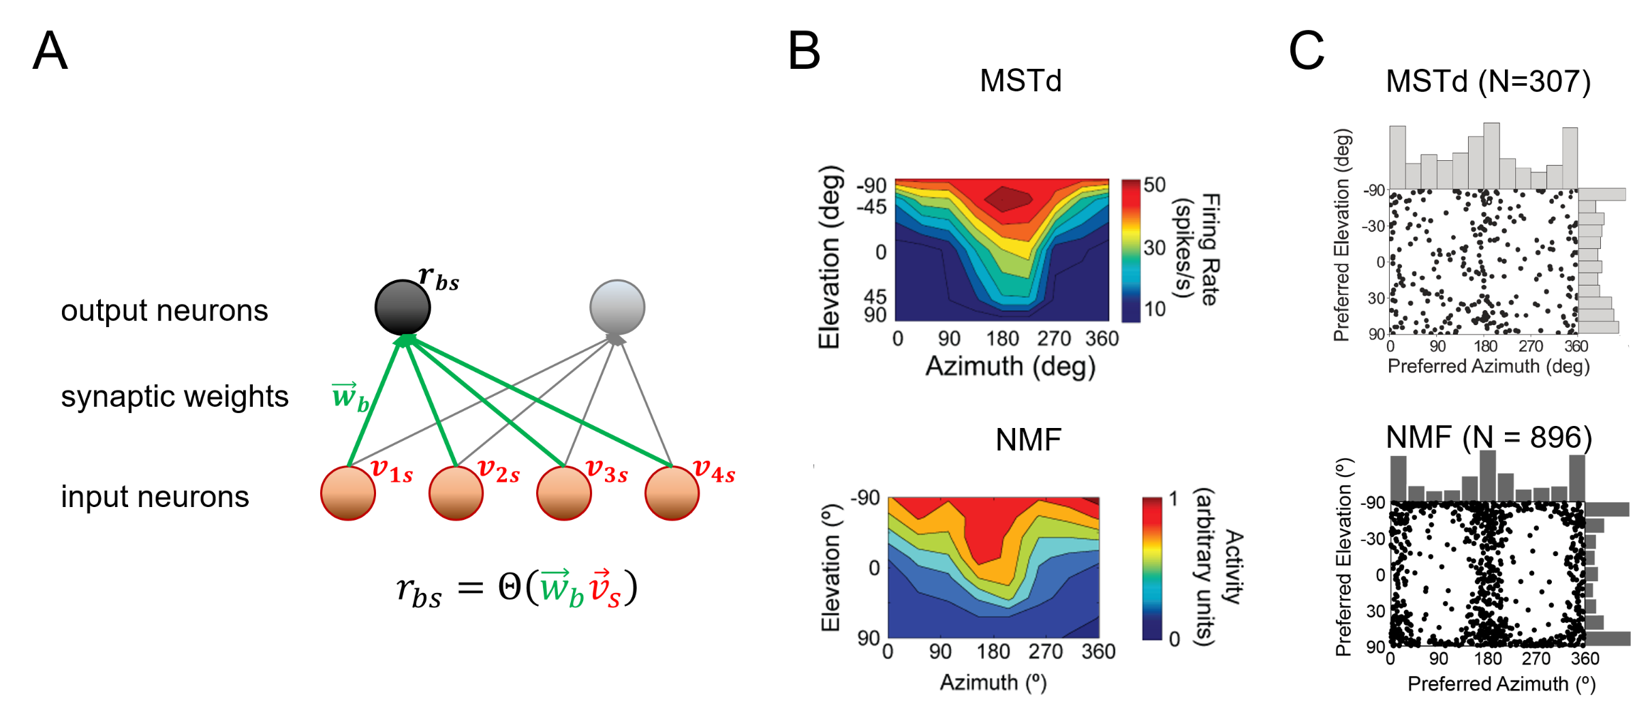
\includegraphics[width=\textwidth]{fig-rev1-responses}
    \caption{\ac{NSC} can predict response properties of biological neurons.
    A) $r_{bs}$ is the response of the $b$-th model output neuron
       to the $s$-th stimulus. $r_{bs}$
       can be calculated from the activity of all
       input neurons (i.e., column $s$ in \textbf{V}), the
       corresponding synaptic weights (i.e., column $b$ in
       $\mathbf{W}$), and a neuronal activation function $\Theta$.
    B) Example of 3D heading tuning for a neuron in macaque
       \ac{MSTd} (top, reprinted from \cite{Takahashi2007}) and a
       simulated neuron (bottom,
       based on the linear response using $\Theta(x)=x$,
       reprinted from \cite{Beyeler2016}).
       Color contour maps show the mean firing rate or model
       activation as a function of azimuth and elevation angles
       of the self-movement direction in 3D.
    C) Classifying simulated akin to biological neuronal responses
       yields distributions of 3D heading preferences akin to 
       macaque \ac{MSTd} (top, reprinted from \cite{Beyeler2016}).
       Each neuron also responded to a preferred direction of 3D
       self-rotation (not shown).}
	\label{fig:NMF|neuronalresponse}
\end{figure}




\subsubsection*{\revise{Visual system}}

\revise{Due to the long history of sparse and efficient coding in vision neuroscience,
the literature is ripe with examples of sparse and parts-based representations
that are in agreement with \ac{NSC}.}

\revise{For example, an \ac{NMF} based model was able to reconstruct
neuronal spike trains in the salamander retina \cite{Onken2016}.}
Following testing on ground truth data, the researchers recorded spikes from in vitro retinal ganglion cells  while the cells were exposed to natural scenes (either still photographs or videos).
They then applied several factorization methods to the data. 
Space-by-time NMF could decompose the data into separate spatial and temporal modules that yielded sparser and more compact representations compared to other techniques, including orthogonal Tucker-2 and basic \ac{NMF}.
\mikeNote{But what does that all mean? Space-by-time NMF? Tucker-2?}
% NMF can also describe patterns of activation observed in retinal ganglion cells (RGCs), which exhibit specific response times and latencies in response to natural images that allow the retina to encode spatial and temporal information embedded in the stimuli. A specific form of NMF, called Tucker-2 or space-by-time NMF, produces separate spatial and temporal basis vectors that most accurately and sparsely describe the spike trains produced by RGCs in the salamander retina \citep{Onken2016}. Nonnegativity constraints, possibly in conjunction with other statistical constraints dependent on the brain region the neurons operate in, may describe the response patterns of neurons in other brain regions that have yet to be tested.


\revise{As discussed above, \ac{NSC} was first demonstrated on simple and
complex cells in \ac{V1} \cite{HoyerHyvarinen2002,Hoyer2003}.
Later, they also modeled V2 hypercomplex cells \cite{Hyvarinen2005}.}
\mikeNote{Expand}

\revise{In our own work \cite{Beyeler2016}, 
we found that simulated neurons in an \ac{NMF} based model 
of \ac{MSTd} responded to simulated optic flow fields
that mimic natural viewing conditions
in much the same way as real neurons in macaque \ac{MSTd}
(Fig.~\ref{fig:NMF|neuronalresponse}B).}
Not only did individual units match response properties of individual neurons
in macaque \ac{MSTd},
but the model was able to recover statistical properties of the \ac{MSTd}
population as a whole, such as a relative overrepresentation of lateral
headings (Fig.~\ref{fig:NMF|neuronalresponse}C).


\subsubsection*{\revise{Auditory cortex}}

\revise{Outside the visual stream, there's lots more stuff.}

http://www.physiology.org/doi/abs/10.1152/jn.00891.2005
\mikeNote{Expand}



\revise{\subsubsection*{Sensory cortex}}
* Evidence from barrel cortex in rats (Spatial organization of neuronal population responses in layer 2/3 of rat barrel cortex)
\mikeNote{If you come across a good figure for any of these areas, I think it would really help us appear more balanced (i.e. less focused on our own work).}

* Auditory cortex (Sparse representation of sounds in the unanesthetized auditory cortex)

* Olfactory cortex (Sparse Incomplete Representations: A Potential Role of Olfactory Granule Cells) and (Causal inference and explaining away in a spiking network)
* Somatosensation?


\revise{\subsubsection*{Motor system}}
* Would it be appropriate to put basal ganglia here? (Information processing, dimensionality reduction and reinforcement learning in the basal ganglia) and (Reinforcement-driven dimensionality reduction–a model for information processing in the basal ganglia)
\mikeNote{Sure, if it flows nicely. Otherwise just make two subsections `basal ganglia' and `motor cortex'.}

* Motor cortex (Rethinking Cortical Organization),(Corticostriatal activity in primary motor cortex of the macaque),(Decoding complete reach and grasp actions from local primary motor cortex populations)


a model known as Reinforcement-Driven Dimensionality Reduction (RDDR)
\mikeNote{revise}
successfully used Hebbian learning to reproduce basal ganglia response patterns associated with reward \cite{BarGad2000}, a function associated with cortico-striato-pallidal circuitry. The authors later applied nonnegativity constraints to the Hebbian learning in the model so that it effectively performed \ac{NMF} on its inputs. The model advanced understanding of the cortico-striato-pallidal loop by capturing behavior of the circuit while explaining the existence of convergent and lateral connections in the region that other models have historically ignored \cite{BarGad2003_Review}. The authors suggest that the basal ganglia uses unsupervised, reward-driven learning to perform dimensionality reduction on cortical inputs for the efficient compression of information in order to plan upcoming actions in the frontal cortex.


\subsubsection*{\revise{Retrosplenial cortex - maybe Archicortex instead?}}
* Hippocampus and Dentate Gyrus (Sparse and specific coding during information transmission between co-cultured dentate gyrus and CA3 hippocampal networks)

* RSC


Analogously, \ac{NSC} can explain response properties
of neurons outside the visual system, 
such as in the \acf{RSC}, an area important for navigation and spatial memory \cite{Miller2014,Nelson2015,VannAggleton2009}.
Neurons in the \ac{RSC} conjunctively encode multiple variables related to the environment and one's position and movement within it, allowing the representation of spatial features of the environment with respect to multiple reference frames \cite{AlexanderNitz2015} (for experimental details, see Supplementary Materials). 

%as determined by an experiment in which rats ran back and forth on a W-shaped track that occupied two different spatial locations within the room in each recording session to test sensitivity to the allocentric reference frame (i.e., track positions $\alpha$ and $\beta$). Outbound and inbound runs were made up of opposite turn sequences (left-right-left (LRL) and right-left-right (RLR), respectively) that corresponded to different sets of trials, which allowed assessment of sensitivity to the egocentric and route-based reference frames. 

However, establishing a mechanistic link between physiological response properties of \ac{RSC} neurons and their underlying representations of space has proved difficult, due to the complexity of their response properties and because inputs to the region are not easily isolated.


We applied NMF to recorded data from the original \ac{RSC} experiment conducted by
Alexander and Nitz \cite{AlexanderNitz2015}. 

%During the experiment, activity from 228 \ac{RSC} neurons was recorded along with four behavioral metrics: linear velocity, angular velocity, head direction, and allocentric position. Using Gaussian and cosine tuning curves, we created idealized input neurons that encoded these four variables. 

By applying \ac{NMF} to the \revise{idealized neural activity}, we were able to replicate
functionality observed in the biological \ac{RSC} (Fig.~\ref{fig:NMF|reconstruction}\revise{C}).
Once again, the dimensionality was reduced from a set of $F = 417$ input neurons to a set of $B = 30$ basis functions.
% \mikeNote{Too soon?}
% The same results were obtained when evolutionary algorithms 
% were used to optimize the metaparameters associated with \ac{STDPH}
% on a population of \acp{SNN} that replicated 
% the same dataset \citep{Rounds2016}.


%    In the case of the \ac{RSC}, the basis vectors that resulted from the NMF model produced activation patterns that could be used to infer behavior, suggesting that the model functions in a manner similar to the biological RSC. Because this region responds to multiple spatial frames of reference (egocentric, route-centric, and allocentric) simultaneously, it is possible to accurately reconstruct the position of an animal within a route situated in a specific part of the environment if neural activity for that route is compared with itself. In contrast, if neural activity associated with the same route but situated in different parts of the room are compared, then the reconstruction of position should be poor (for more details, see \citep{AlexanderNitz2015}), showing that the \ac{RSC} distinguishes routes that have different allocentric positions in space. We found that the activity patterns computed using the NMF basis vectors yielded qualitatively similar results when subjected to the same analysis.

% The results were also consistent for the \ac{RSC}. In the neurophysiological dataset, experimentally observed neurons were classified into three broad categories: 
% % these 3 are so incredibly, excruciatingly wordy 
% 1) those that were insensitive to turn-based actions performed by the rats running along the track but nonetheless exhibited complex and robust firing patterns, 2) those that were sensitive purely to turning behaviors performed by the rats such that they responded exclusively to left or right turns, and 3) neurons that demonstrated turn type selectivity, but with increased firing associated with specific instances of the preferred turn type based on their position in the turn sequence associated with the route regardless of the route's location in allocentric space. When \ac{NMF} was applied to the behavioral variables encoded by idealized input neurons, the resulting basis vectors could be categorized into the same functional categories and followed the same approximate distributions as in the experimental dataset (Fig.  \ref{fig:NMF|neuronalresponse}B).


% In the case of the \ac{RSC}, the basis vectors that resulted from the NMF model produced activation patterns that could be used to infer behavior, suggesting that the model functions in a manner similar to the biological RSC. Because this region responds to multiple spatial frames of reference (egocentric, route-centric, and allocentric) simultaneously, it is possible to accurately reconstruct the position of an animal within a route situated in a specific part of the environment if neural activity for that route is compared with itself. In contrast, if neural activity associated with the same route but situated in different parts of the room are compared, then the reconstruction of position should be poor (for more details, see \citep{AlexanderNitz2015}), showing that the \ac{RSC} distinguishes routes that have different allocentric positions in space. We found that the activity patterns computed using the NMF basis vectors yielded qualitatively similar results when subjected to the same analysis.






% The sparsity and nonnegativity constraints of the \ac{NSC} seem to extract similarities between neuronal firing patterns that result in
% consistent and stable representations, 
% while other statistical methods of dimensionality reduction 
% instead extract differences in firing patterns, thus capturing underlying representations of the data that are less stable and consistent, and are often less sparse. However, the exact implementation of dimensionality reduction in any given part of the brain might vary with the structure, and connectivity of the region.









These remarkable findings where \ac{NSC} can account for neuronal response properties across a wide range of
brain areas and modalities strongly suggests that these 
 representations emerge due to the pressure to find efficient, perceptually and behaviorally relevant stimulus features.
At the population level, \ac{NSC} promotes representations in which
neurons act as generalists rather than specialists,
allowing for the simultaneous encoding of multiple variables of interest
(e.g., heading, eye rotation velocity in \ac{MSTd} \cite{Beyeler2016})
with respect to multiple frames of reference
(e.g., egocentric, route-based in \ac{RSC} \cite{Rounds2016}).
Among the advantages of such basis function representations
\cite{Poggio1990,PougetSejnowski1997,PougetSnyder2000}
(also called mixed-selectivity representations
\cite{Eichenbaum2017,Fusi2016,Barak2013})
are robustness to noise as well as the ability to decode various variables of interest
through a linear combination of neuronal responses.

% The fact that  \ac{NSC} can account for the response properties of neurons in a diverse set of brain regions that play fundamentally different roles in behavior and cognition is somewhat astounding since individual brain regions are often assumed to have their own unique methods of handling their unique inputs. Evidence for the prevalence of such a computation raises some fundamental questions about how neurons have evolved to help us survive. In particular, these findings suggest that neurons are not, in fact, specialized for particular kinds of computations or functionality, and that it is more advantageous for neurons to be capable of handling all information flexibly. Several researchers have argued that 'mixed selectivity' is a fundamental feature of neurons in higher cortical regions \citep{Eichenbaum2017,Fusi2016,Barak2013}, because higher cognition requires that neurons encode multiple task-relevant variables. Such generalizability is an expected property of neurons under the NSC framework, since the algorithm aims to encode as much information about the stimulus as possible while using the fewest number of neurons to do it. If optimizing these metrics, it is expected that neurons would not be specialized for certain behaviors or inputs, and would instead be equally likely to respond to all types of inputs. This is further supported by evidence showing that sparsity levels amidst populations of neurons demonstrating mixed selectivity helps to control the tradeoff between generalization and discrimination \citep{Barak2013}.

